
\begin{frame}
\frametitle{Organization}
\PraesentationSchriftgroesseGross
\begin{itemize}
    \item RGB-D Data
    \item Basic Idea of Direct Visual Odometry
    \item Warping Function
    \item MAP Estimation
    \item Residual Weighting
    \item Image Pyramid
\end{itemize}

\end{frame}
\clearpage

\begin{frame}
\frametitle{RGB-D Data}

A RGB-image $\mathcal{I}_i$ with the corresponding depth image $\mathcal{Z}_i$ indicating the pixel-to-camera-plane distance. \\

Dataset used in this project: the TUM Dataset (https://vision.in.tum.de/data/datasets/rgbd-dataset) \\[\baselineskip]

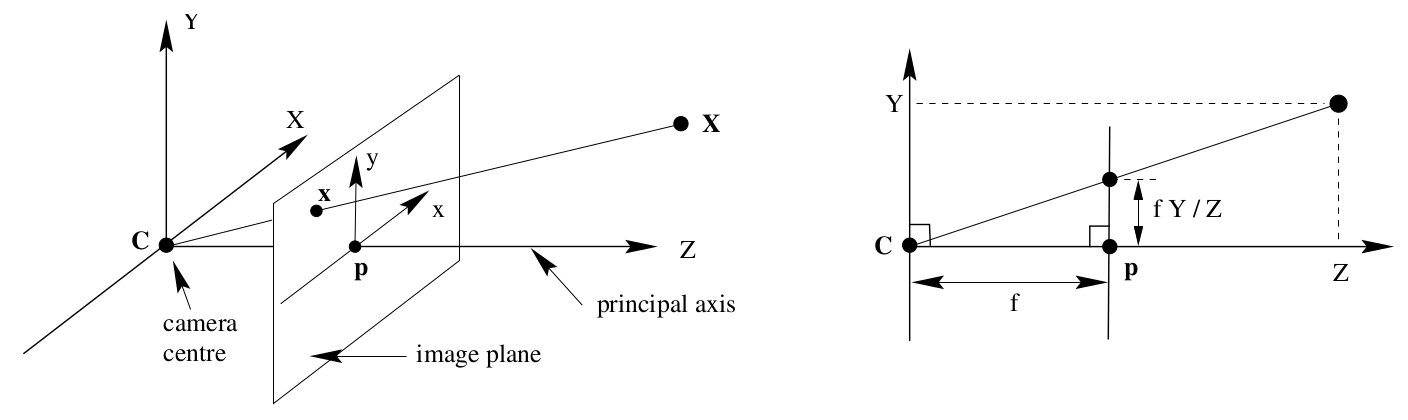
\includegraphics[width=\textwidth]{Bilder/depth.png}

\end{frame}
\clearpage

\begin{frame}
\frametitle{RGB-D Data}

A RGB-image $\mathcal{I}_i$ with the corresponding depth image $\mathcal{Z}_i$ indicating the pixel-to-camera-plane distance. \\

Dataset used in this project: the TUM Dataset (https://vision.in.tum.de/data/datasets/rgbd-dataset) \\[\baselineskip]

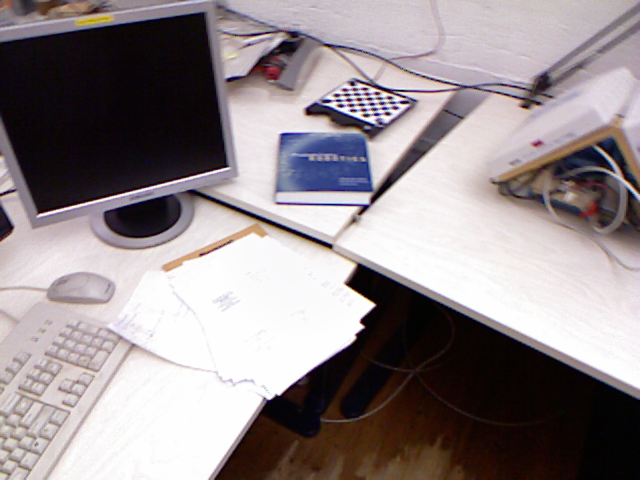
\includegraphics[height=.5\paperheight]{Bilder/rgbd-rgb.png}
\hspace{6.5mm}%
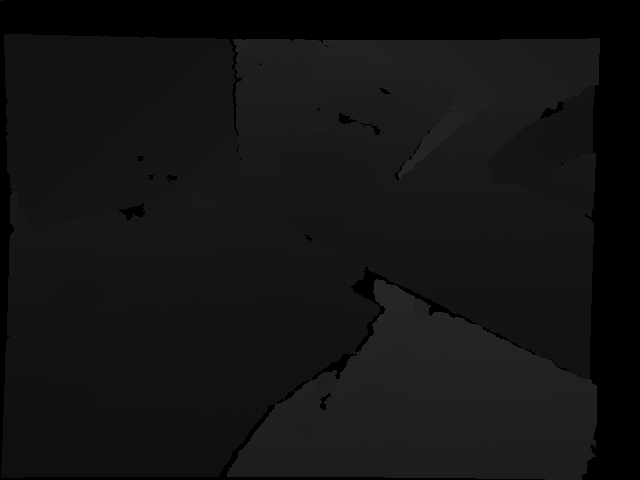
\includegraphics[height=.5\paperheight]{Bilder/rgbd-depth.png}

\end{frame}
\clearpage

\begin{frame}
\frametitle{Basic Idea of Direct Visual Odometry}

\vspace{1.5em}
\begin{multicols}{2}
    \begin{itemize}
        \item Consider at each time step a successive pair of frames $(\mathcal{I}_1, \mathcal{Z}_1)$ and $(\mathcal{I}_2, \mathcal{Z}_2)$
        \vspace{0.5em}\item Warp each pixel $\mathbf{x}$ from the coordinate of $\mathcal{I}_1$ to that of $\mathcal{I}_2$ using the warping function $\mathbf{x}' = \tau(\boldsymbol{\xi}, \mathbf{x})$
        \vspace{0.5em}\item A world point $\mathbf{p}$ observed by two cameras is assumed to yield the same brightness, i.e. $$\mathcal{I}_{1}(\mathbf{x}) = \mathcal{I}_{2}(\tau(\boldsymbol{\xi}, \mathbf{x}))$$
        \vfill \item Minimize the overall loss function based on residuals $r_i(\boldsymbol{\xi}) := \mathcal{I}_2\left(\tau\left(\boldsymbol{\xi}, \mathbf{x}_i\right)\right)-\mathcal{I}_1\left(\mathbf{x}_i\right)$ by solving the MAP estimation to obtain camera motion $\boldsymbol{\xi}$
        
    \end{itemize}
    \vfill\columnbreak
    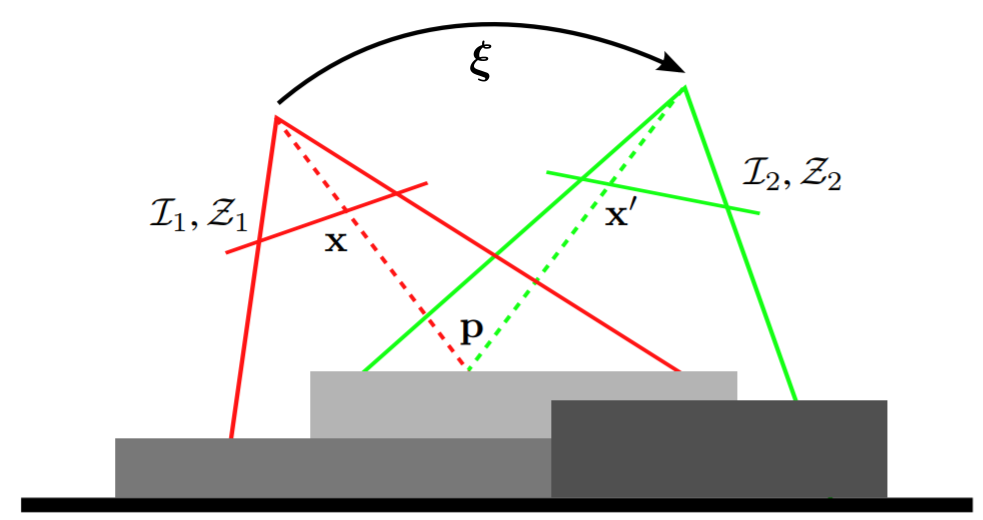
\includegraphics[width=\columnwidth]{Bilder/warping.png}%
\end{multicols}

\end{frame}
\clearpage


\begin{frame}
\frametitle{Warping Function}

\vspace{1.5em}
\begin{multicols}{2}
    \begin{itemize}
        \item Unprojection:
        $$\mathbf{p} = \pi^{-1}\left(\mathbf{x}, \mathcal{Z}_1(\mathbf{x})\right) = \mathcal{Z}_{1}(\mathbf{x})\left(\frac{u+c_x}{f_x}, \frac{v+c_y}{f_y}, 1\right)^{\top}$$
        \vfill\item Transformation:
        $$T(g(\boldsymbol{\xi}), \mathbf{p})=R \mathbf{p}+\mathbf{t}$$
        \vfill\item Projection:
        $$\pi(T(g, \mathbf{p}))=\left(\frac{f_x X}{Z}-c_x, \frac{f_y Y}{Z}-c_y\right)^{\top}$$
        \vfill\item Summing up:
        $$\tau(\boldsymbol{\xi}, \mathbf{x}) =\pi(T(g(\boldsymbol{\xi}), \mathbf{p})) = \pi\left(T\left(g(\boldsymbol{\xi}), \pi^{-1}\left(\mathbf{x}, \mathcal{Z}_1(\mathbf{x})\right)\right)\right)$$
    \end{itemize}
    \vfill\columnbreak
    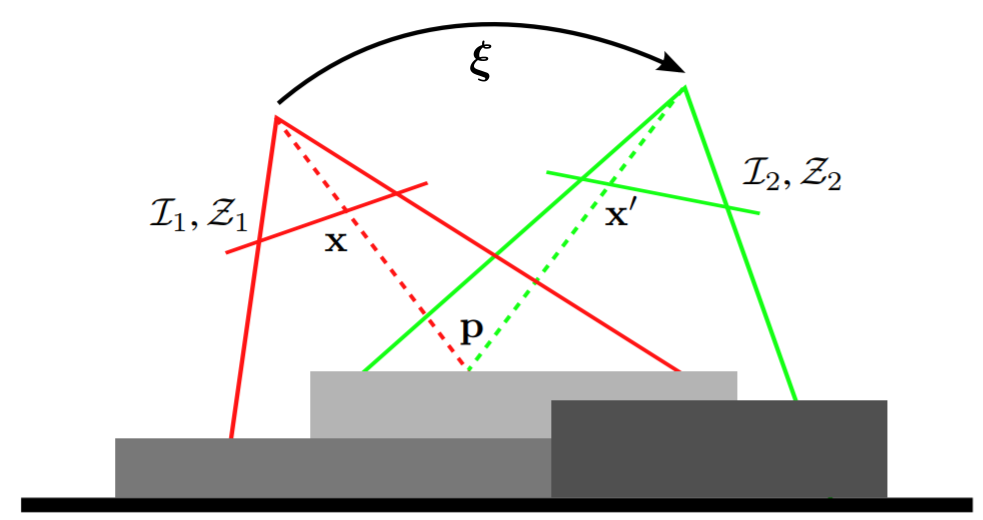
\includegraphics[width=\columnwidth]{Bilder/warping.png}%
\end{multicols}

\end{frame}
\clearpage

\begin{frame}
\frametitle{MAP Estimation}

\begin{itemize}
    \item Reminder: residual $r_i(\boldsymbol{\xi}) := \mathcal{I}_2\left(\tau\left(\boldsymbol{\xi}, \mathbf{x}_i\right)\right)-\mathcal{I}_1\left(\mathbf{x}_i\right)$
    \vspace{1em}\item A posteriori likelihood of camera motion $\boldsymbol{\xi}$:
    $$p(\boldsymbol{\xi} | \mathbf{r})=\frac{p(\mathbf{r} | \boldsymbol{\xi}) p(\boldsymbol{\xi})}{p(\mathbf{r})}$$
    \item Setting derivatives w.r.t $\boldsymbol{\xi}$ to zero and working out some math:
    $$\boldsymbol{\xi}_{\mathrm{MAP}}=\arg \min _{\boldsymbol{\xi}} \sum_{i} w\left(r_{i}\right)\left(r_{i}(\boldsymbol{\xi})\right)^{2}$$
    \item Weighted least squares problem: Gauss-Newton, Levenberg-Marquardt, ...
    \vfill
\end{itemize}

\end{frame}
\clearpage

\begin{frame}
\frametitle{Residual Weighting}

\vspace{1.5em}
\begin{multicols}{2}
    \begin{itemize}
        \item Reminder:$$\boldsymbol{\xi}_{\mathrm{MAP}}=\arg \min _{\boldsymbol{\xi}} \sum_{i} w\left(r_{i}\right)\left(r_{i}(\boldsymbol{\xi})\right)^{2}$$
        \vfill\item If the residuals are normally distributed, then all $w(r_i)$ are identical, leading to a non-weighted least squares minimization problem.
        \vfill\item A t-distribution can better describe the observed distribution of residuals.
        \vfill\item The influence of too large residuals (usually outliers) can be better suppressed.
    \end{itemize}
    \vfill\columnbreak
    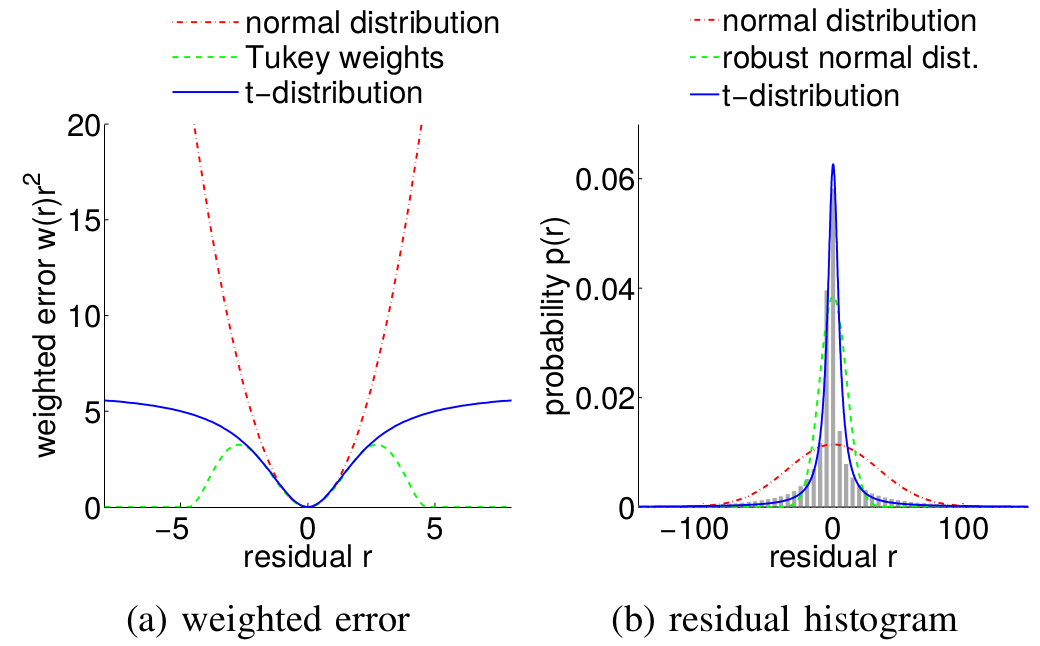
\includegraphics[width=\columnwidth]{Bilder/distribution.png}%
\end{multicols}

\end{frame}
\clearpage

\begin{frame}
\frametitle{Residual Weighting}

Example: a hand (outlier pixels) moving through the scene \\[\baselineskip]

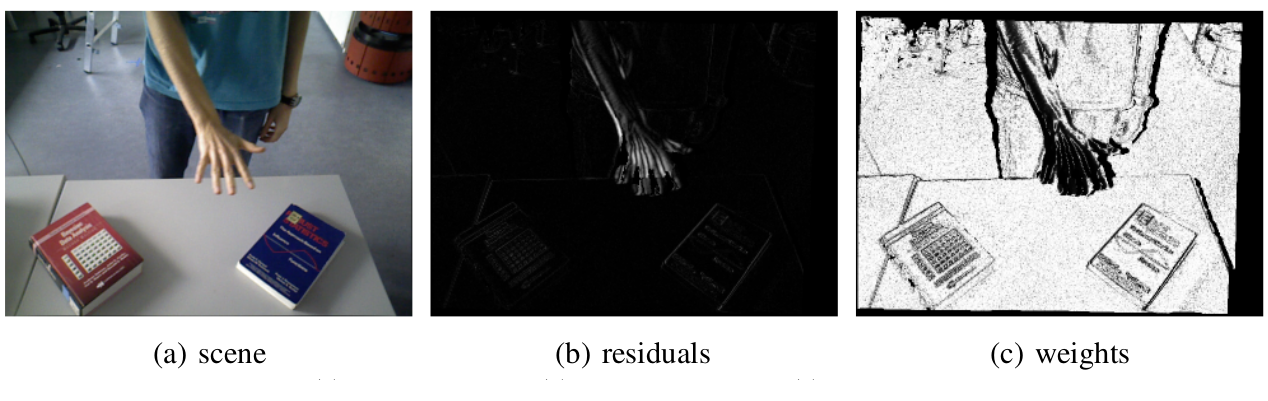
\includegraphics[width=\textwidth, height=.55\textheight]{Bilder/weighting.png}%

\end{frame}
\clearpage

\begin{frame}
\frametitle{Image Pyramid}

Coarse-to-fine scheme:
\vspace{-1em}
\begin{itemize}
    \item Image pyramid that half the image resolution at each level
    \item Estimated camera motion at each level as initialization for the next level.
\end{itemize}

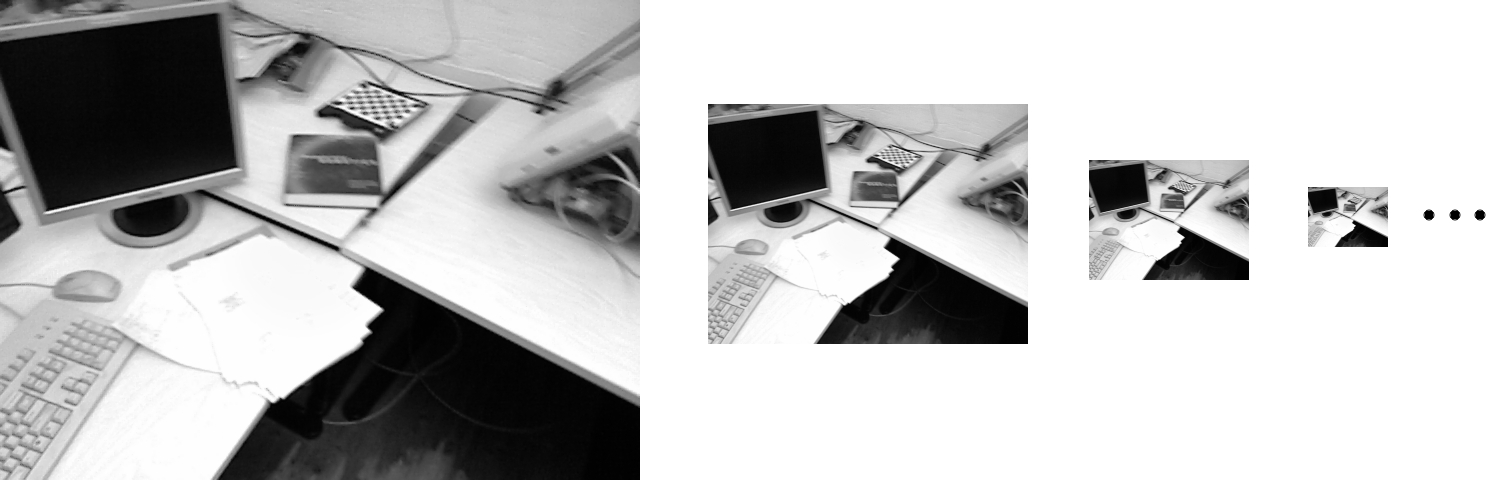
\includegraphics[width=\textwidth, height=.5\textheight]{Bilder/pyramid.jpg}%

\end{frame}
\clearpage

\begin{frame}
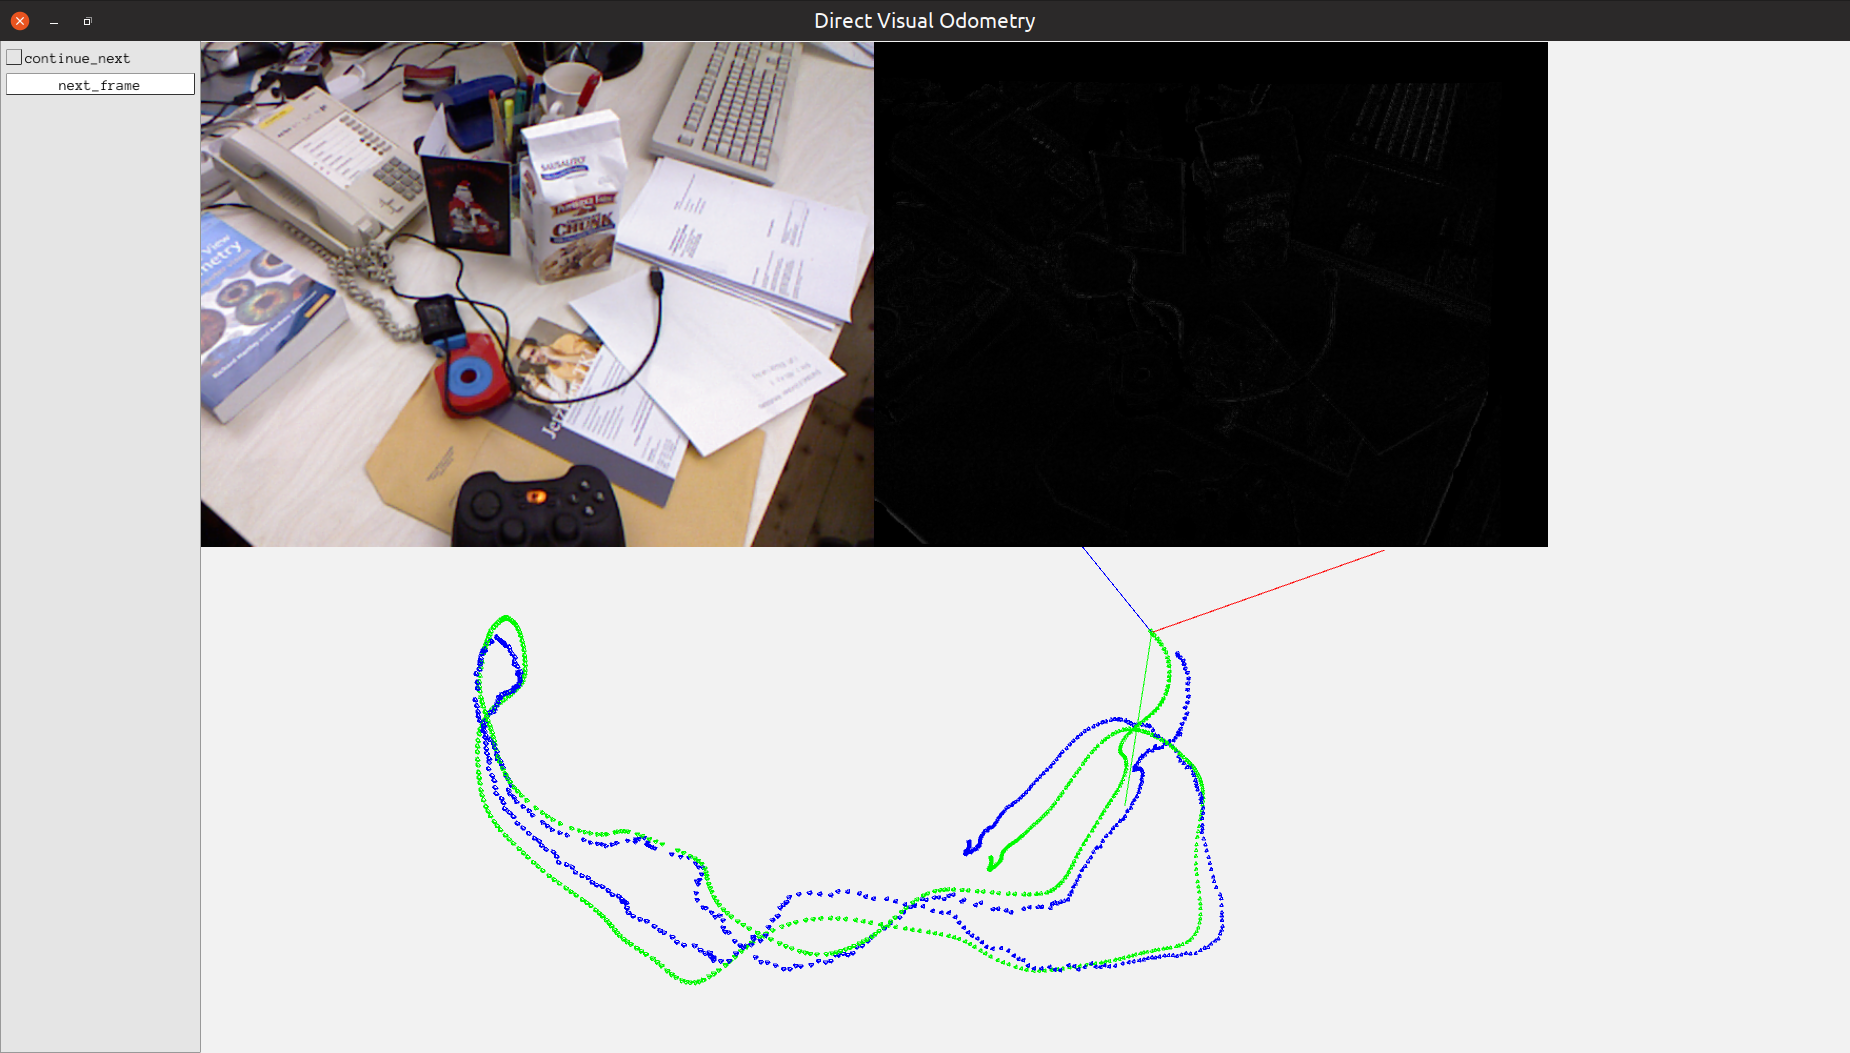
\includegraphics[width=0.92\textwidth]{Bilder/result.png}%

\end{frame}
\clearpage

\begin{frame}
\frametitle{Thank you for your attention! \\ \vspace{2em}Any questions?}

\end{frame}
\clearpage
